\documentclass{article}

% these packages let you do math
\usepackage{amsmath}
\usepackage{amssymb}

% we need these packages for fancy R tables
\usepackage{booktabs}
\usepackage{float}
\usepackage{colortbl}
\usepackage{xcolor}

% these packages play with the spacing/margins of the document. Uncomment the commands on lines 16 and 17 to see what they do.
\usepackage{a4wide}
\usepackage{setspace}
\usepackage{geometry}
\usepackage{parskip}
%\doublespacing
%\geometry{margin=1.5in}

% this package helps us with including images. Setting the graphics path makes it easier to refer to things in the \includegraphics command.
\usepackage{graphicx}
\graphicspath{ {../figures/} }

% make some hyperlinks using the \href command
\usepackage{hyperref}
\hypersetup{
    colorlinks=true,
    linkcolor=black,
    urlcolor=blue
}

% set the author, title, and date of the document. \maketitle adds it to the document.
\author{Yu Xia}
\title{My Paper on NLSY97 Data}
\date{Sping 2022}

\begin{document}
\maketitle

\section{Introduction}

This paper talks about incarceration status of different gender and race. In order to examine the difference between different categories, this paper use the data provided by National Longitudinal Survey. I choose NLSY97, which interviewed many American youth in 1997. There are many information about education, employment, marrraige, etc. This paper focuses on the incarceration status in the year 2002.

Firstly, I filter out wrong data. Incarceration data of pervious months are dropped as well. Thus, all incarceration I'm looking at happened in 2002. Thereafter, I categorise the data by race and gender, according to the original data. Meanwhile, I  take the sum of each person's incarceration variable. It shows how many months this person spent incarcerated. For example, If the sum is 9, this person spent 9 months incarcerated. Then I take the mean time of incarceration by each group. As shown below, this paper compare different catefories by figure, simple econometrics model and tables. 

\newpage

\section{Interpretation}

Wherein we do tables and graphs. To include the graph we made in ggplot, we create the \texttt{figure} environment. The `H' option tells LaTeX to `hold' the position of the figure instead of positioning it somewhere else. I use the \texttt{caption} command to add a caption{\textemdash}although I also put a title on the plot in ggplot so you would typically choose one or the other. I use the \texttt{label} command after the caption to add a label. Then in my paper I can use the \texttt{ref} command and LaTeX knows I am referring to Figure \ref{fig:graph}.


\begin{figure}[H]
    \begin{center}
        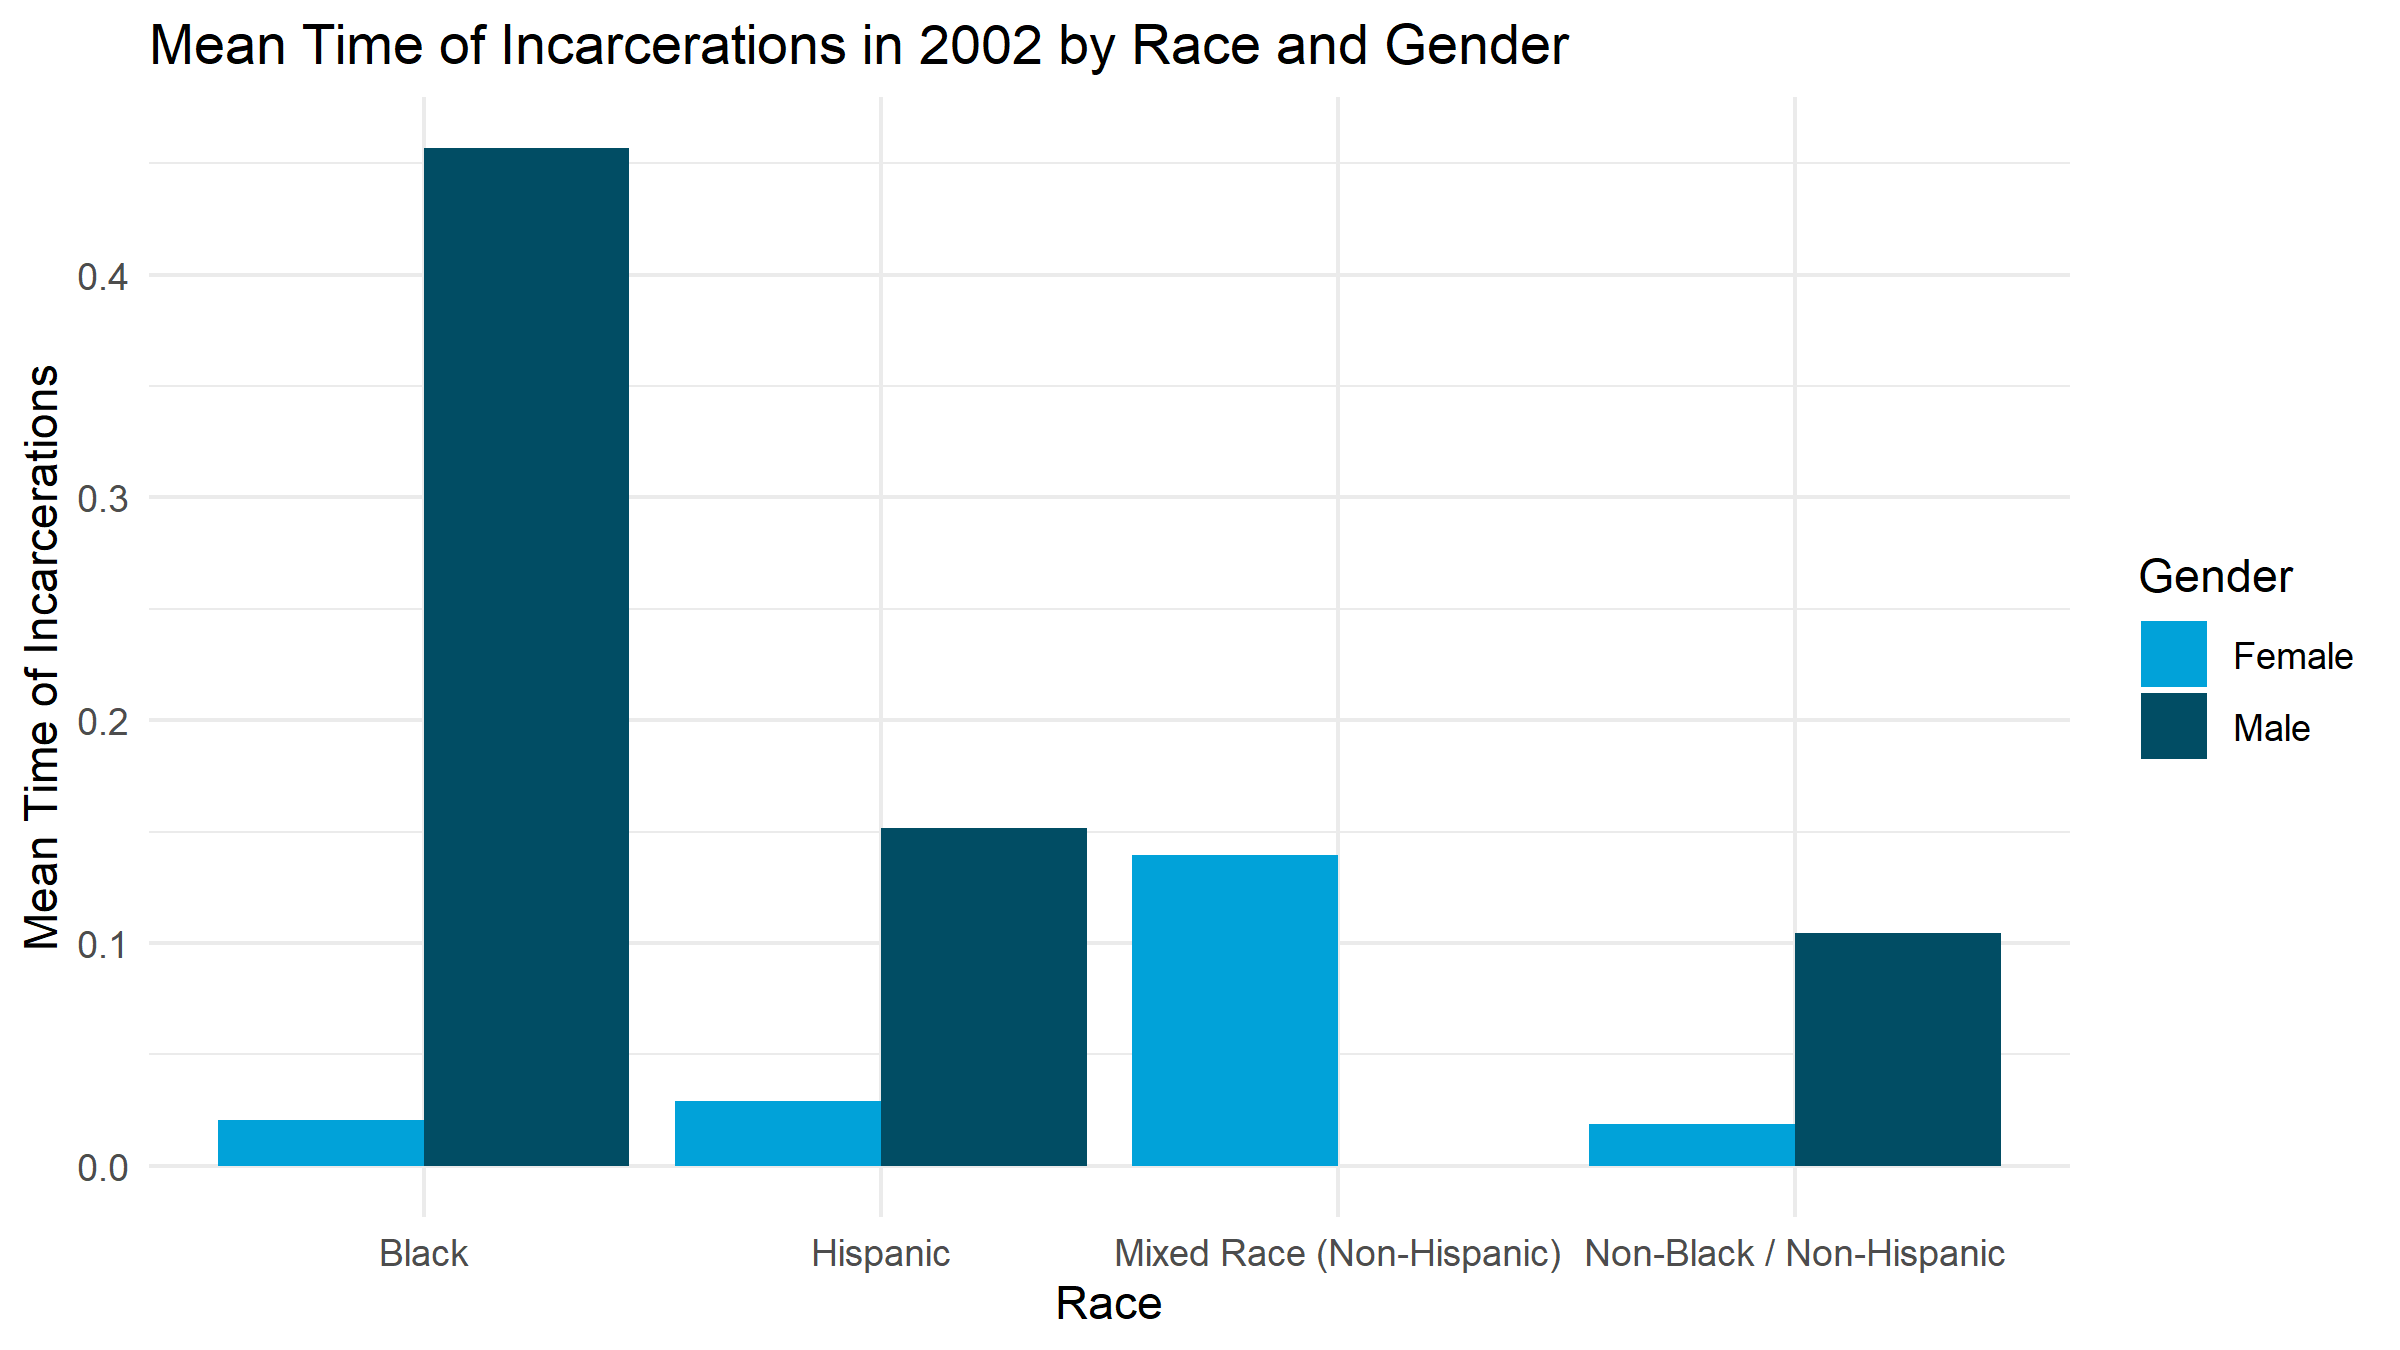
\includegraphics[width=.85\textwidth]{incarcerations_by_racegender}
    \end{center}
    \caption{Mean Number of Incarcerations in 2002 by Race and Gender (this is the LaTeX caption, not the ggplot title)}
    \label{fig:graph}
\end{figure}


Tables are somewhat easier, since \texttt{kableExtra} and \texttt{stargazer} generate LaTeX code that is ready to just ``copy-paste'' into our document. The \texttt{label} argument in the R code is the label that the table will have in the tex output, if you want to \texttt{ref} it.

\begin{table}[H]

\caption{\label{tab:tab:summarystats}Mean incarceration time in 2002 by Race and Gender}
\centering
\begin{tabular}[t]{lrrrr}
\toprule
Gender & Black & Hispanic & Mixed Race Non Hispanic & Non Black Non Hispanic\\
\midrule
\cellcolor{gray!6}{Female} & \cellcolor{gray!6}{0.0205832} & \cellcolor{gray!6}{0.0292208} & \cellcolor{gray!6}{0.1395349} & \cellcolor{gray!6}{0.0186501}\\
Male & 0.4568007 & 0.1514841 & 0.0000000 & 0.1044343\\
\bottomrule
\end{tabular}
\end{table}



% Table created by stargazer v.5.2.2 by Marek Hlavac, Harvard University. E-mail: hlavac at fas.harvard.edu
% Date and time: ����, 2�� 16, 2022 - 18:06:17
\begin{table}[!htbp] \centering 
  \caption{Regression Output. Omitted category is Black Females.} 
  \label{tab:regression} 
\begin{tabular}{@{\extracolsep{5pt}}lc} 
\\[-1.8ex]\hline 
\hline \\[-1.8ex] 
 & \multicolumn{1}{c}{\textit{Dependent variable:}} \\ 
\cline{2-2} 
\\[-1.8ex] & Incarcerations in 2002 \\ 
\hline \\[-1.8ex] 
 Hispanic & $-$0.149$^{***}$ \\ 
  & (0.037) \\ 
  & \\ 
 Mixed Race (Non-Hispanic) & $-$0.163$^{**}$ \\ 
  & (0.081) \\ 
  & \\ 
 Non-Black / Non-Hispanic & $-$0.179$^{***}$ \\ 
  & (0.033) \\ 
  & \\ 
 Male & 0.183$^{***}$ \\ 
  & (0.021) \\ 
  & \\ 
 Constant & 0.148$^{***}$ \\ 
  & (0.024) \\ 
  & \\ 
\hline \\[-1.8ex] 
Observations & 8,984 \\ 
R$^{2}$ & 0.014 \\ 
Adjusted R$^{2}$ & 0.013 \\ 
Residual Std. Error & 0.999 (df = 8979) \\ 
F Statistic & 31.172$^{***}$ (df = 4; 8979) \\ 
\hline 
\hline \\[-1.8ex] 
\textit{Note:}  & \multicolumn{1}{r}{$^{*}$p$<$0.1; $^{**}$p$<$0.05; $^{***}$p$<$0.01} \\ 
\end{tabular} 
\end{table} 


\end{document}